\documentclass{report}
\usepackage{amsmath}
\usepackage{graphicx}
\graphicspath{ {./} }
\begin{document}
\part{Question One}
\section{Question}
We want to combine three transformations into one by multiplying them. The transformation S should be applied second; the transformation T should be applied first; the transformation R should be applied third. Write the product of the three transformations showing the order in which they should be multiplied.
\section{Answer}
\begin{enumerate}
	\item Translation
	\item Scaling
	\item Rotation
\end{enumerate}
$\begin{bmatrix}
x^1 \\
y^1 \\
z^1
\end{bmatrix}
=
\underset{Translation}{\begin{bmatrix}
1 & 0 & 0 & a \\
0 & 1 & 0 & b \\
0 & 0 & 1 & c \\
0 & 0 & 0 & 1
\end{bmatrix}}
\underset{Scaling}{\begin{bmatrix}
a & 0 & 0 & 0 \\
0 & b & 0 & 0 \\
0 & 0 & c & 0 \\
0 & 0 & 0 & 1
\end{bmatrix}}
\underset{Rotation}{\begin{bmatrix}
\cos\theta & -a\sin\theta & 0 & 0 \\
\sin\theta & \cos\theta & 0 & 0 \\
0 & 0 & 1 & 0 \\
0 & 0 & 0 & 1
\end{bmatrix}}
\begin{bmatrix}
x \\
y \\
z \\
1 \\
\end{bmatrix}
\\
\begin{bmatrix}
a & 0 & 0 & a \\
0 & b & 0 & b \\
0 & 0 & c & c \\
0 & 0 & 0 & 1
\end{bmatrix}
\begin{bmatrix}
\cos\theta & -a\sin\theta & 0 & 0 \\
\sin\theta & \cos\theta & 0 & 0 \\
0 & 0 & 1 & 0 \\
0 & 0 & 0 & 1
\end{bmatrix}
\begin{bmatrix}
x \\
y \\
z \\
1 \\
\end{bmatrix}
\\
\underset{ResultingMatrix}{\begin{bmatrix}
\cos\theta & -a\sin\theta & 0 & a \\
\sin\theta & \cos\theta & 0 & b \\
0 & 0 & 1 & c \\
0 & 0 & 0 & 1
\end{bmatrix}
\begin{bmatrix}
x \\
y \\
z \\
1 \\
\end{bmatrix}}
$
\part{Question Two}
\section{Question}
Write the code that carries out the following steps. You may assume that the appropriate imports have been provided.
\section{Answer}
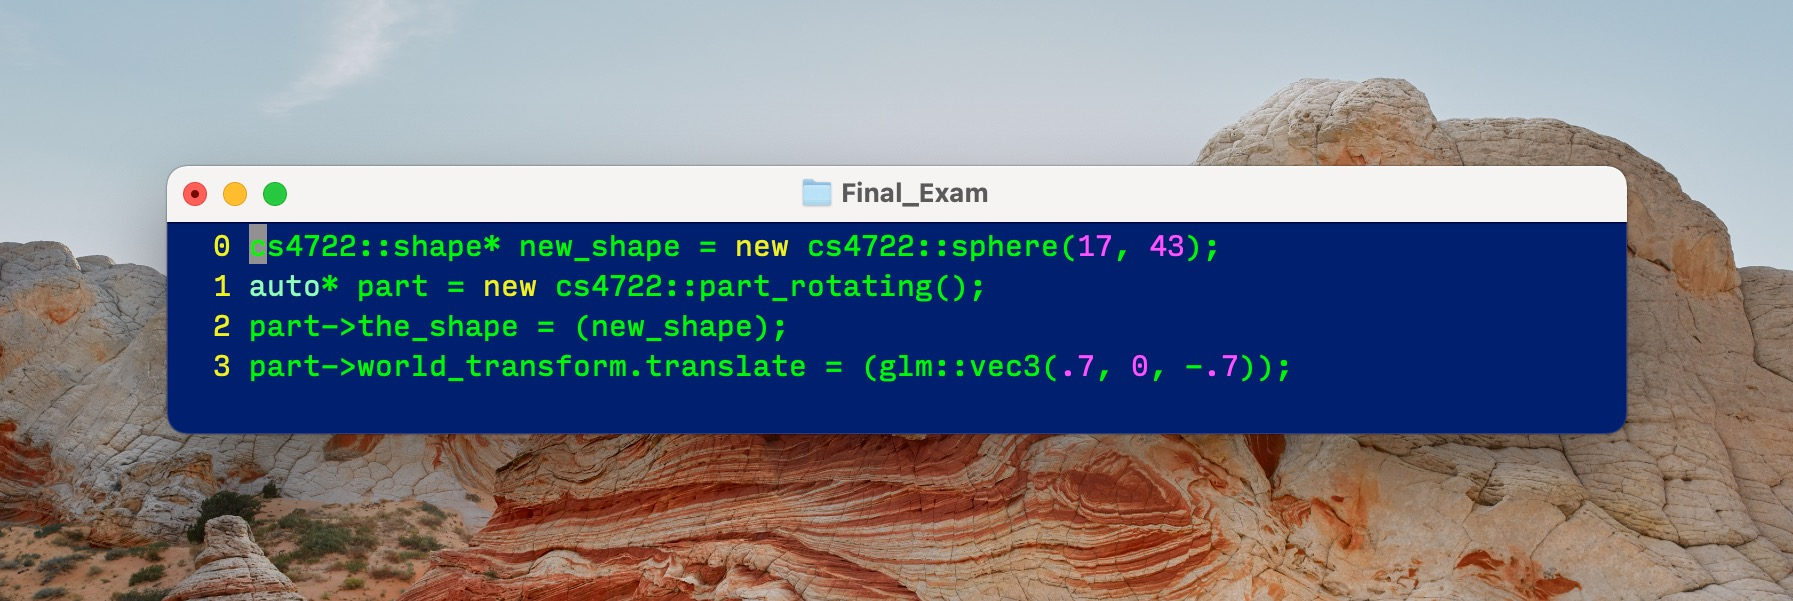
\includegraphics[width=1.0\textwidth]{question_two}
\part{Question Three: Data Memory}
\section{Question}
We want to render a geometric figure which is modeled using 38 triangles.
As with almost all of our examples, he figure will be drawn using gl triangles mode. This question is about measuring the memory used to store the vertex data.
\subsection{ How many vertices will be used to represent each triangle?}
\subsection{Answer}
\subsection{ Using the standard way we have represented vertex positions in our code examples, how many float values will be used to represent each vertex position?
}
\subsection{Answer}
\subsection{ How many float values in all will it take to represent all the vertex positions for the figure?
}
\subsection{Answer}
\subsection{ How many bytes will that take to store all this position data?
}
\subsection{Answer}
\subsection{ In the examples where colors were assigned to vertices, each color was represented by a cs4722::color object. How many bytes does it take to store the data (r, g, b, and a components) of a cs4722::color object?}
\subsection{Answer}
\subsection{ How many bytes would it take to store all of the color data assigned to the vertices of this figure?}
\subsection{Answer}
\part{Question Four: Pipeline}
\section{Question}
Each part below describes a stage or a process in the standard OpenGL rendering pipeline. Your answer is to name the pipeline stage or process.
\subsection{ For a single geometric primitive, determines the pixels that are covered by the primitive.}
\subsection{Answer}
Primitive Setup
\subsection{ Subdivides shapes more complex than primitives into standard primitive shapes}
\subsection{Answer}
Culling and clipping
\subsection{ For a single vertex, does some processing and outputs a vertex to the later stages}
\subsection{Answer}
Vertex Shader
\subsection{ Takes one or more vertices and creates a geometric primitive from them}
\subsection{Answer}
Geometry Shader
\subsection{ For a single pixel, does some processing and outputs a color for that pixel}
\subsection{Answer}
Fragment Processing
\part{Question Five: Drawing Modes}
\section{Question}
The image to the below shows six points stored in the GPU buffer. The list of points starts with the black point, lower left, and continue around clockwise: black, red, green, blue, magenta, cyan. These points can be used to draw triangles or lines or points' in various ways, depending on the drawing mode. TRIANGLES or LINES for example.- -> For each picture below, tell which drawing mode was used to produce that picture. Each of the seven drawing modes available is used in one of the parts.

\subsection{POINTS}
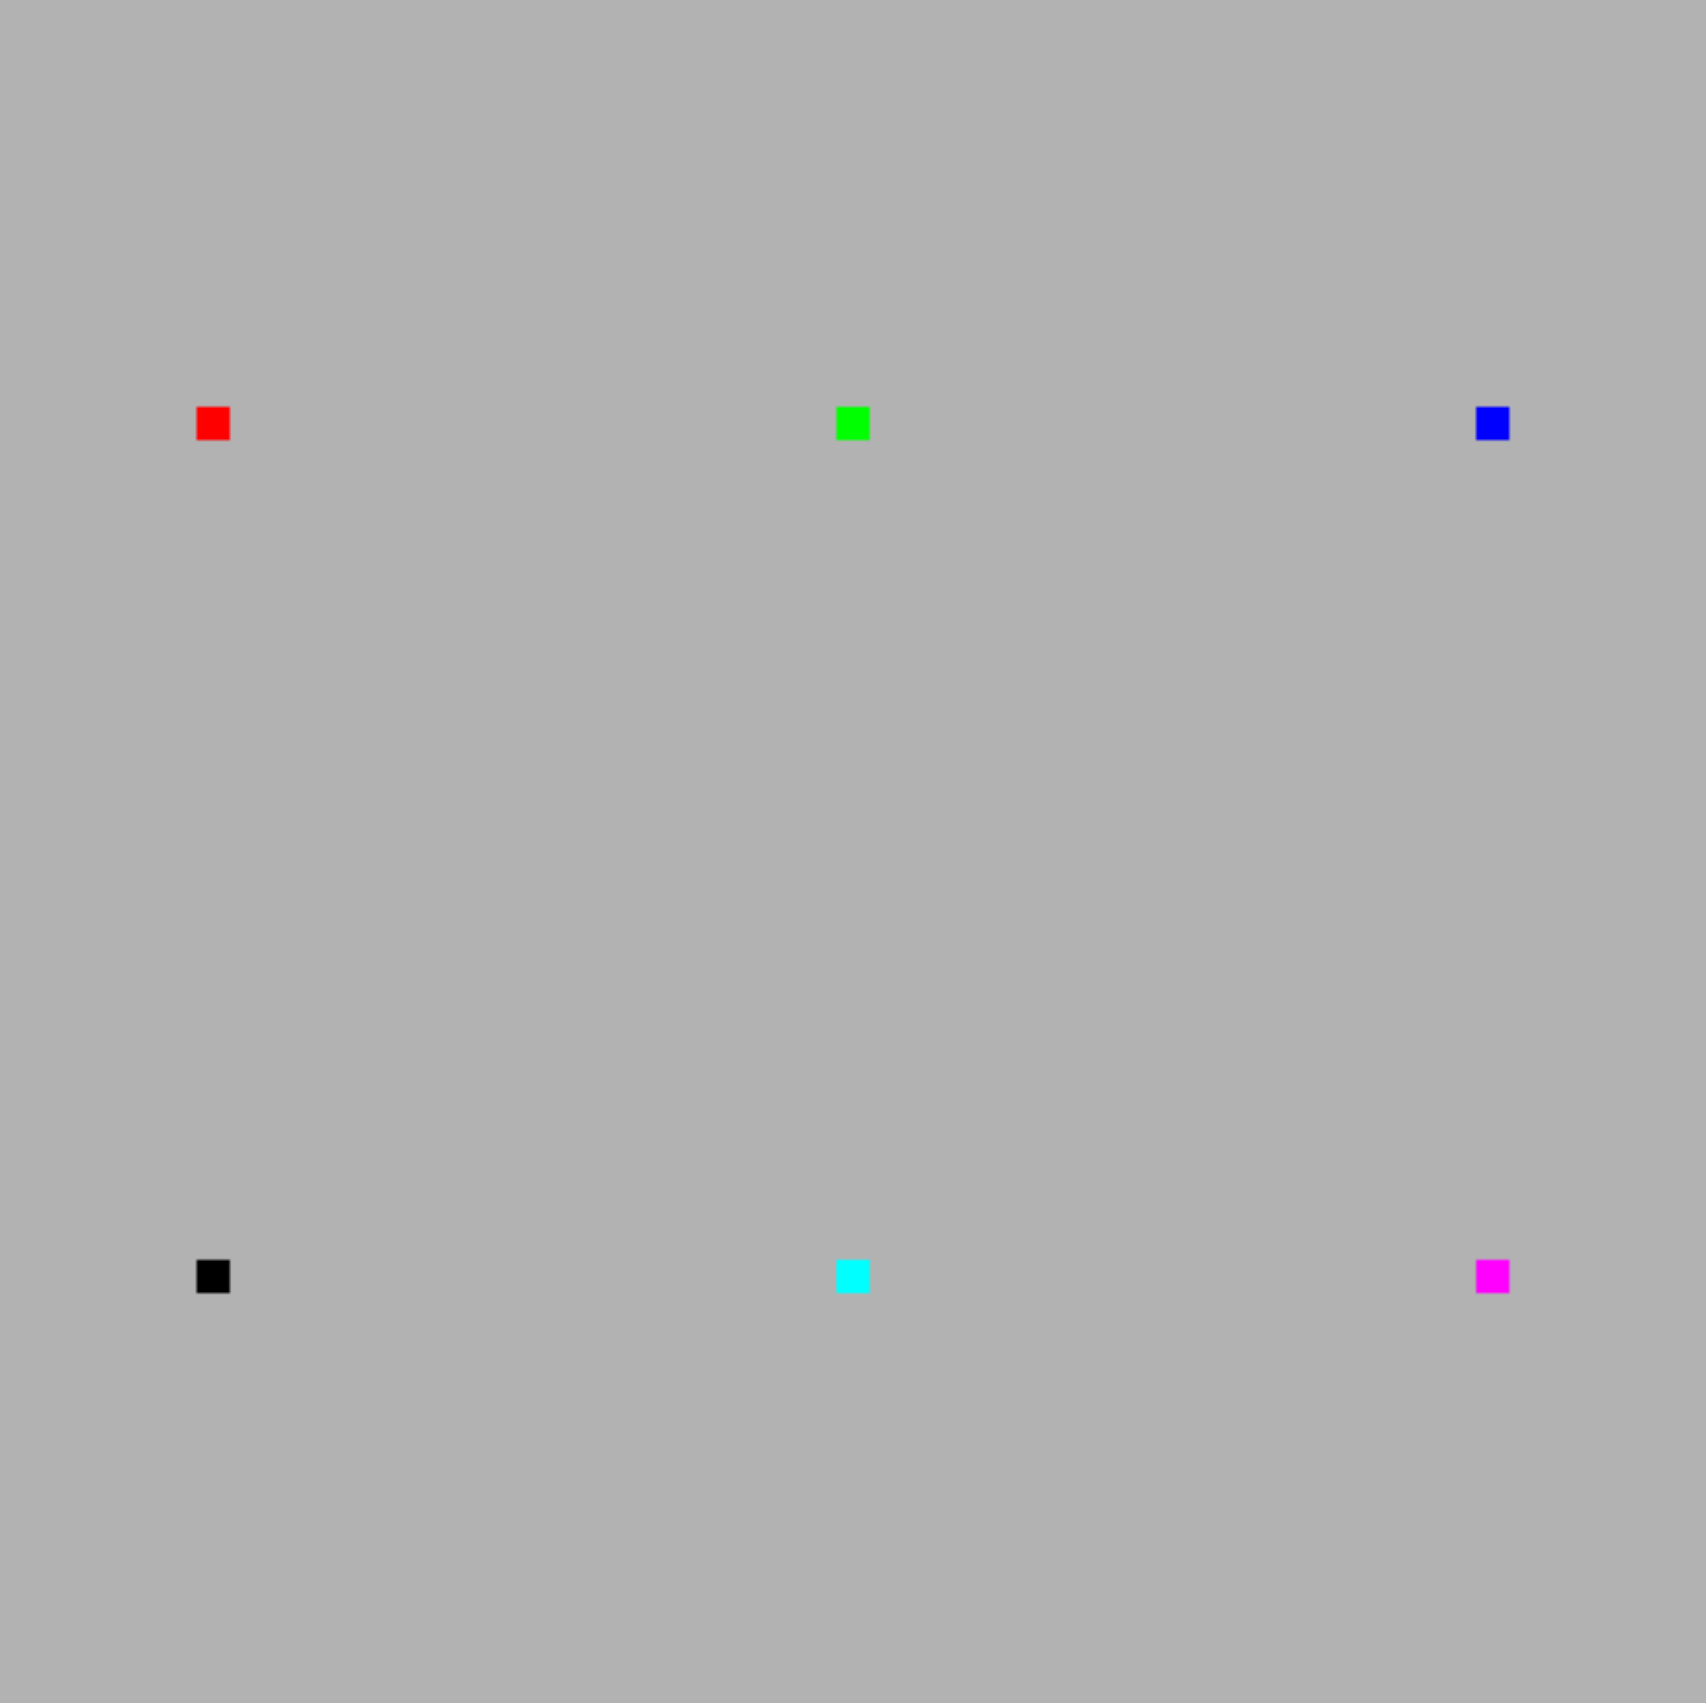
\includegraphics[width=1.0\textwidth]{Image_1}
\subsection{LINE STRIP}
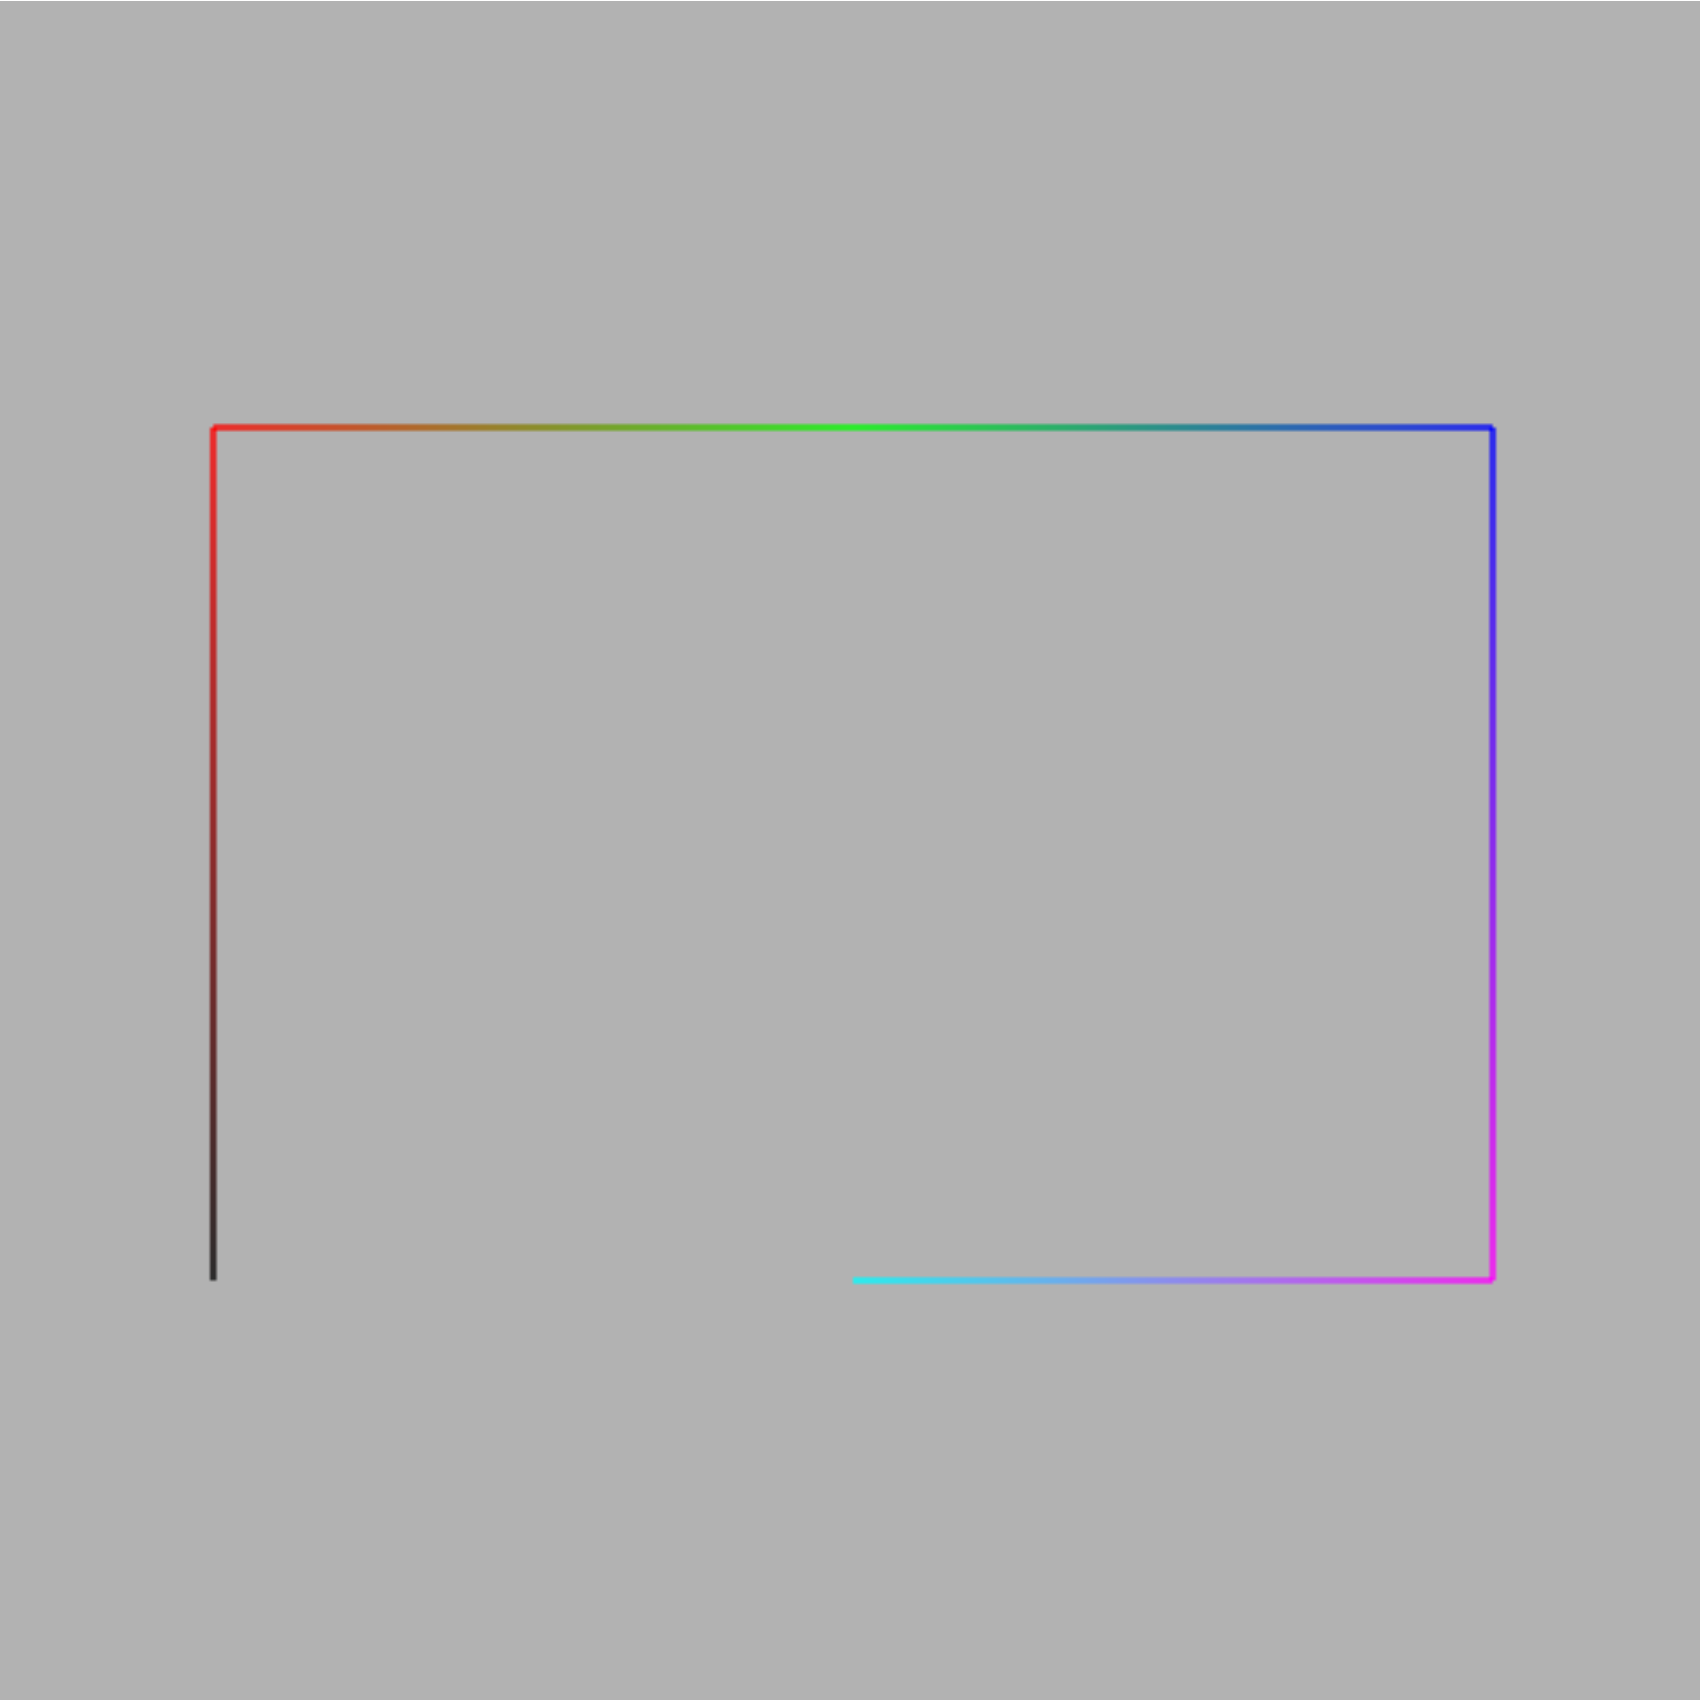
\includegraphics[width=1.0\textwidth]{Image_0}
\subsection{LINE LOOP}
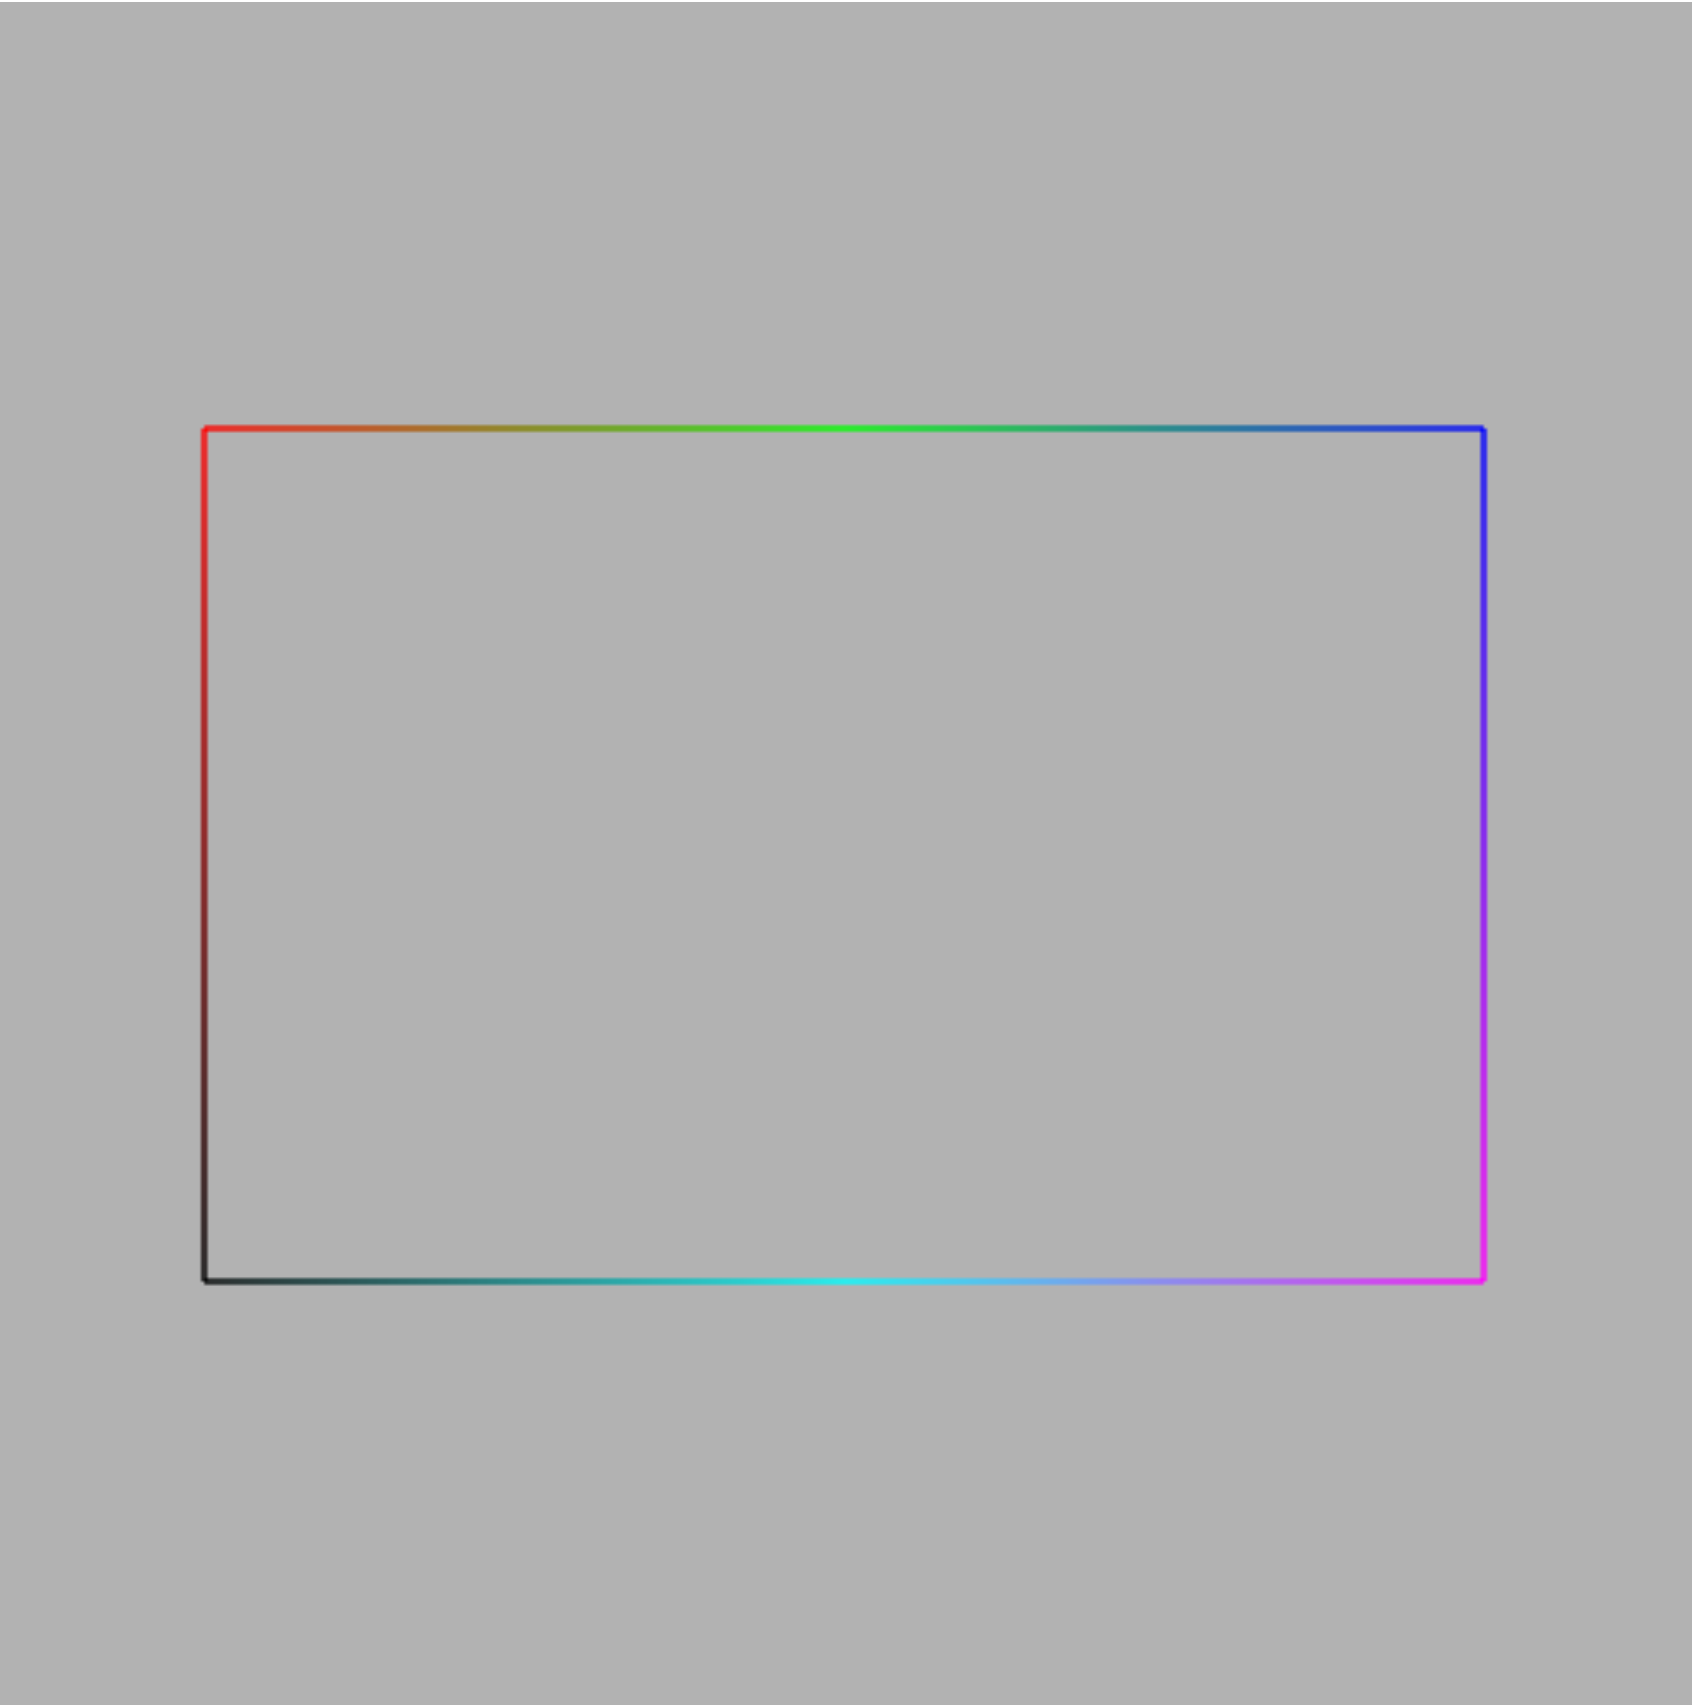
\includegraphics[width=1.0\textwidth]{Image_2}
\subsection{TRIANGLE STRIP}
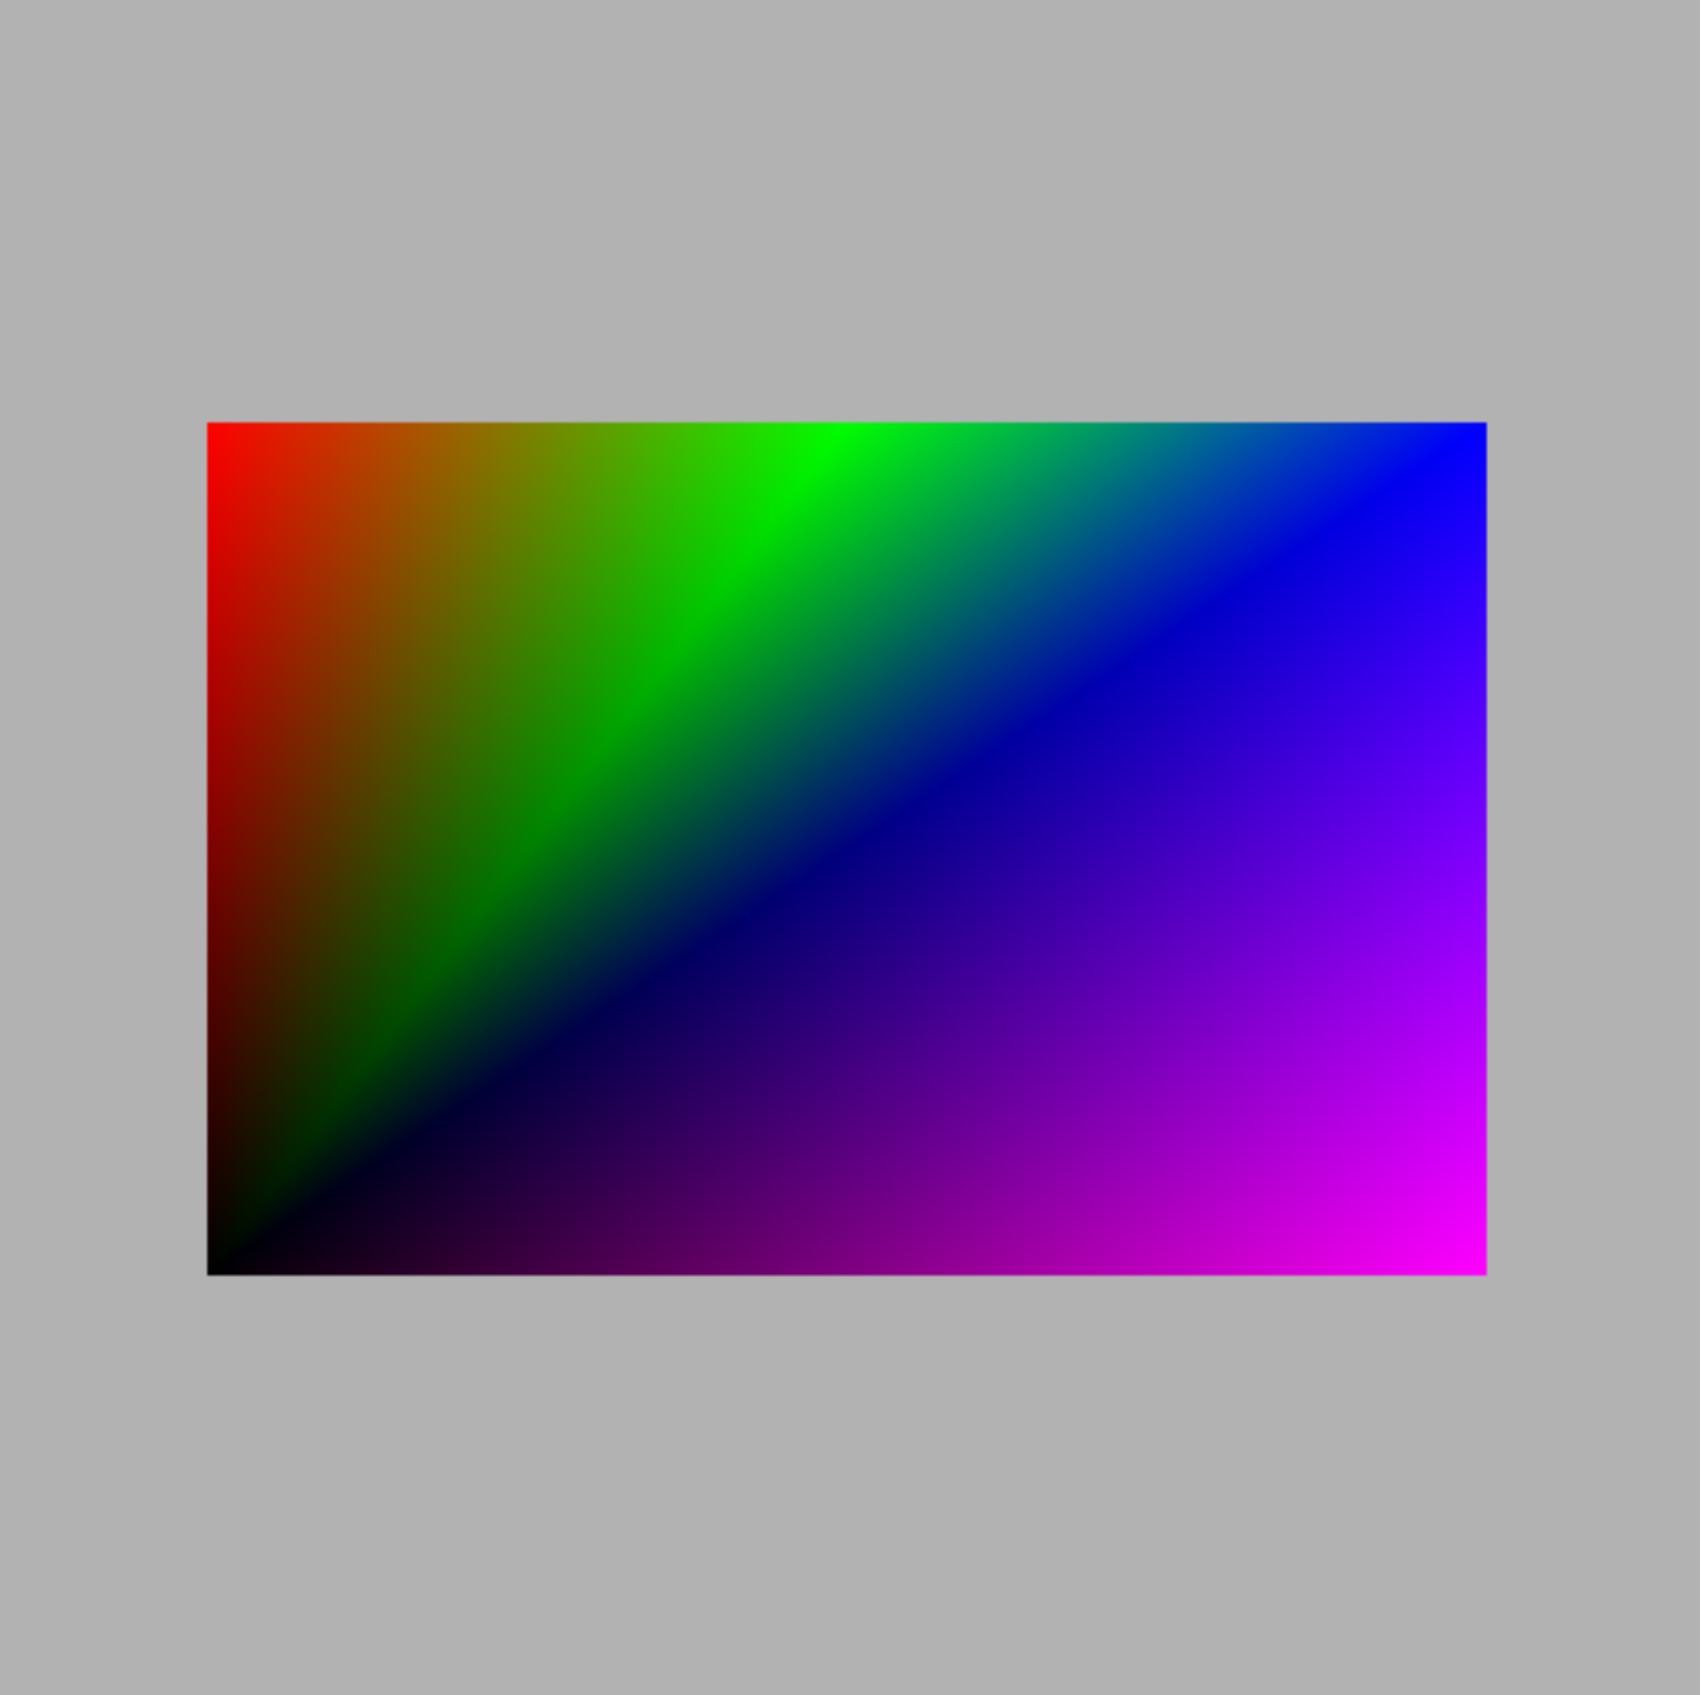
\includegraphics[width=1.0\textwidth]{Image_3}
\subsection{LINES}
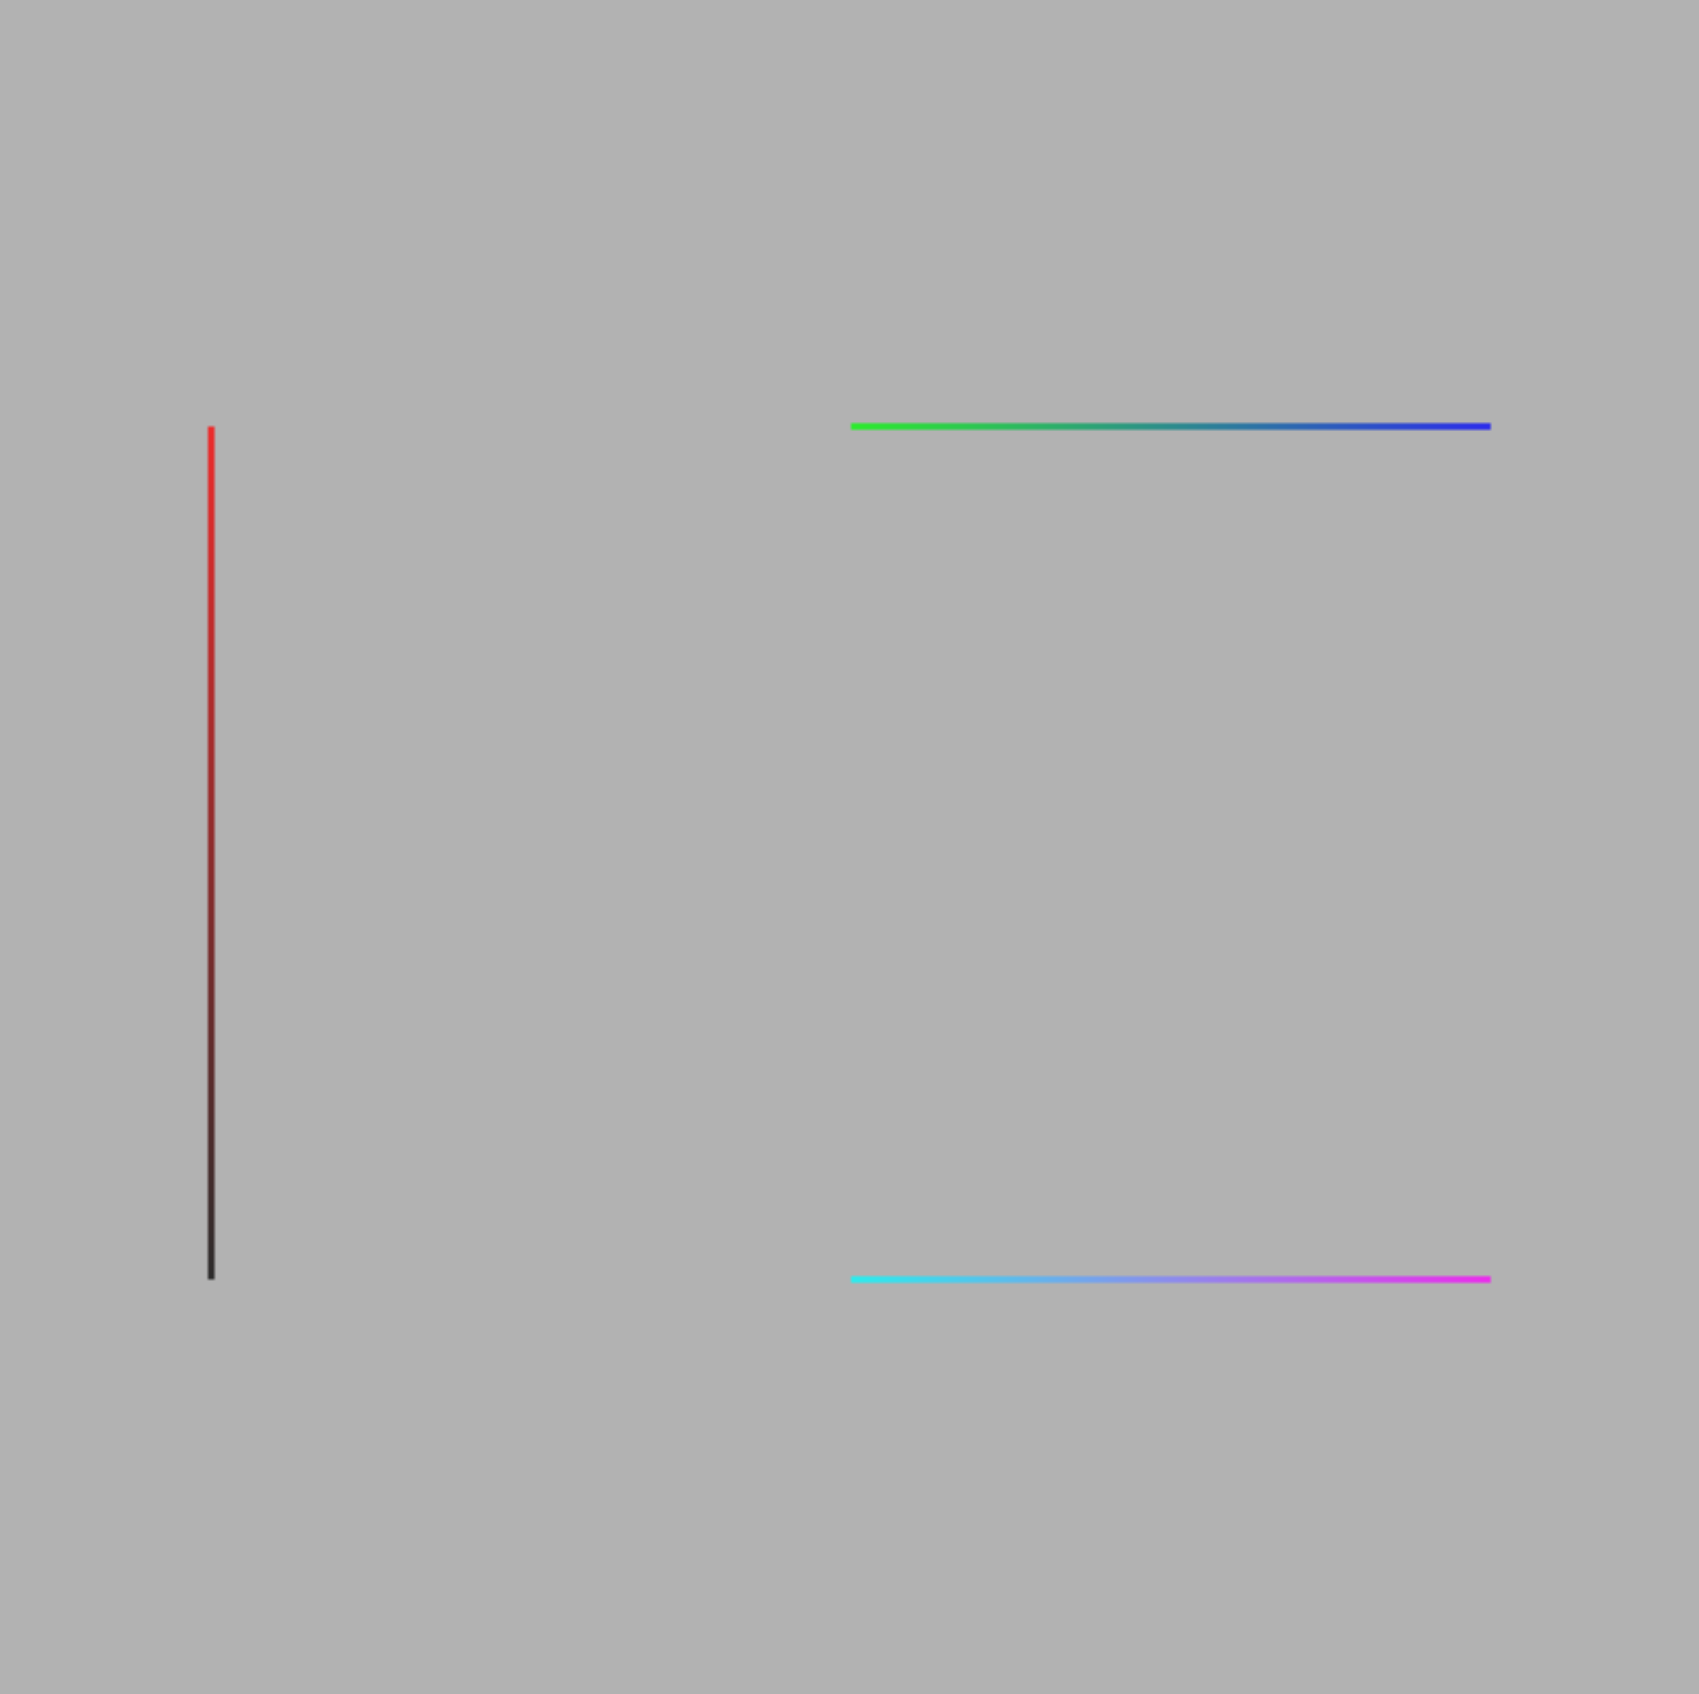
\includegraphics[width=1.0\textwidth]{Image_4}
\subsection{TRIANGLES}
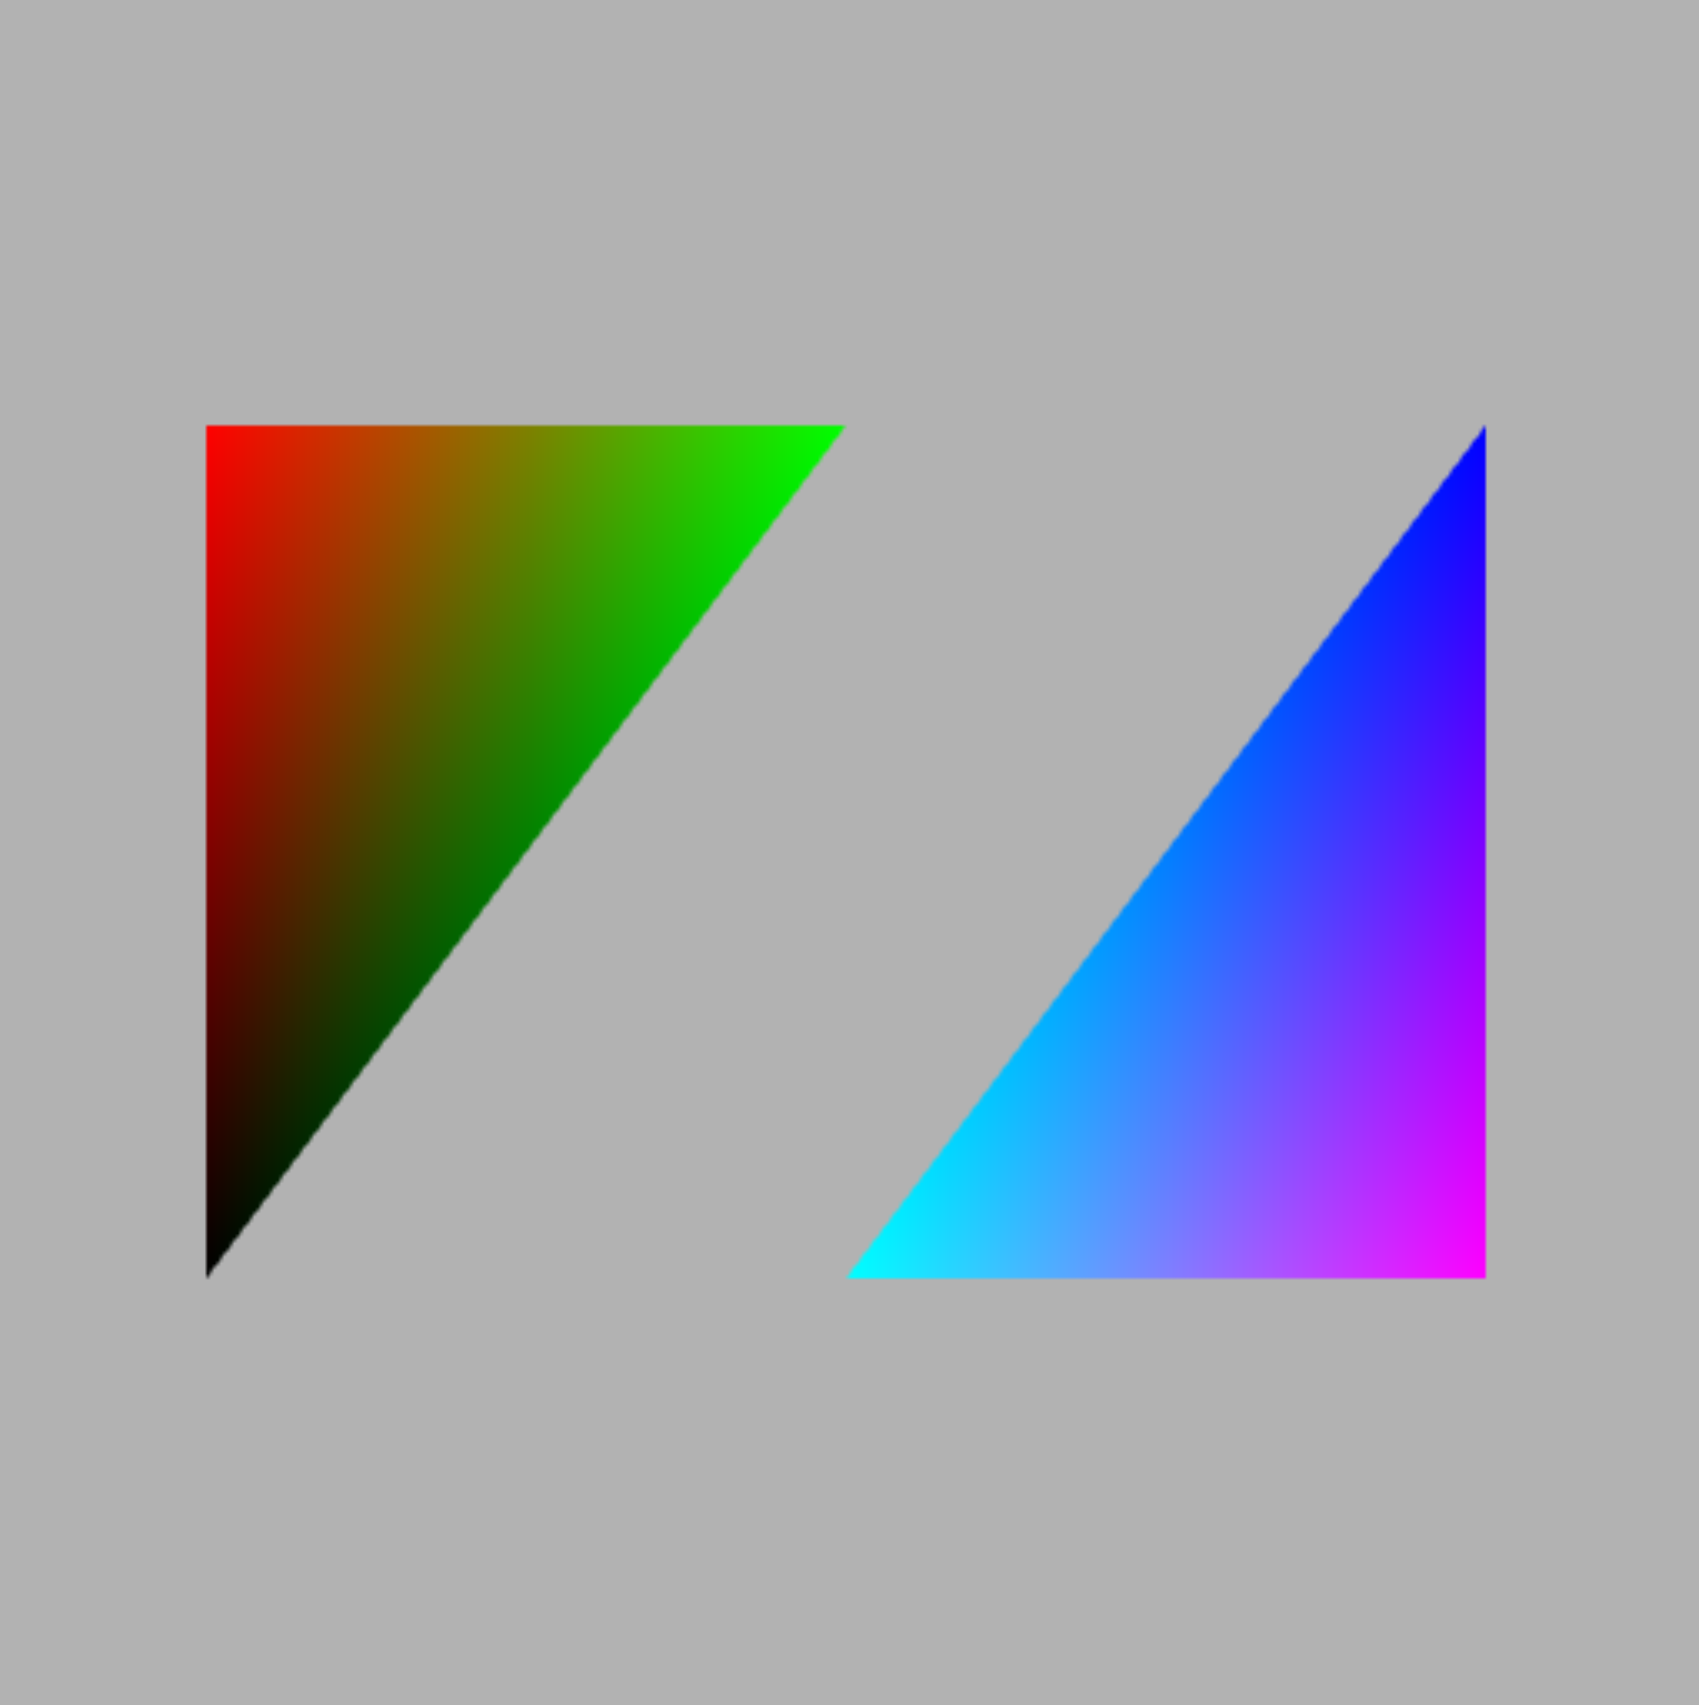
\includegraphics[width=1.0\textwidth]{Image_5}
\subsection{TRIANGLE FAN}
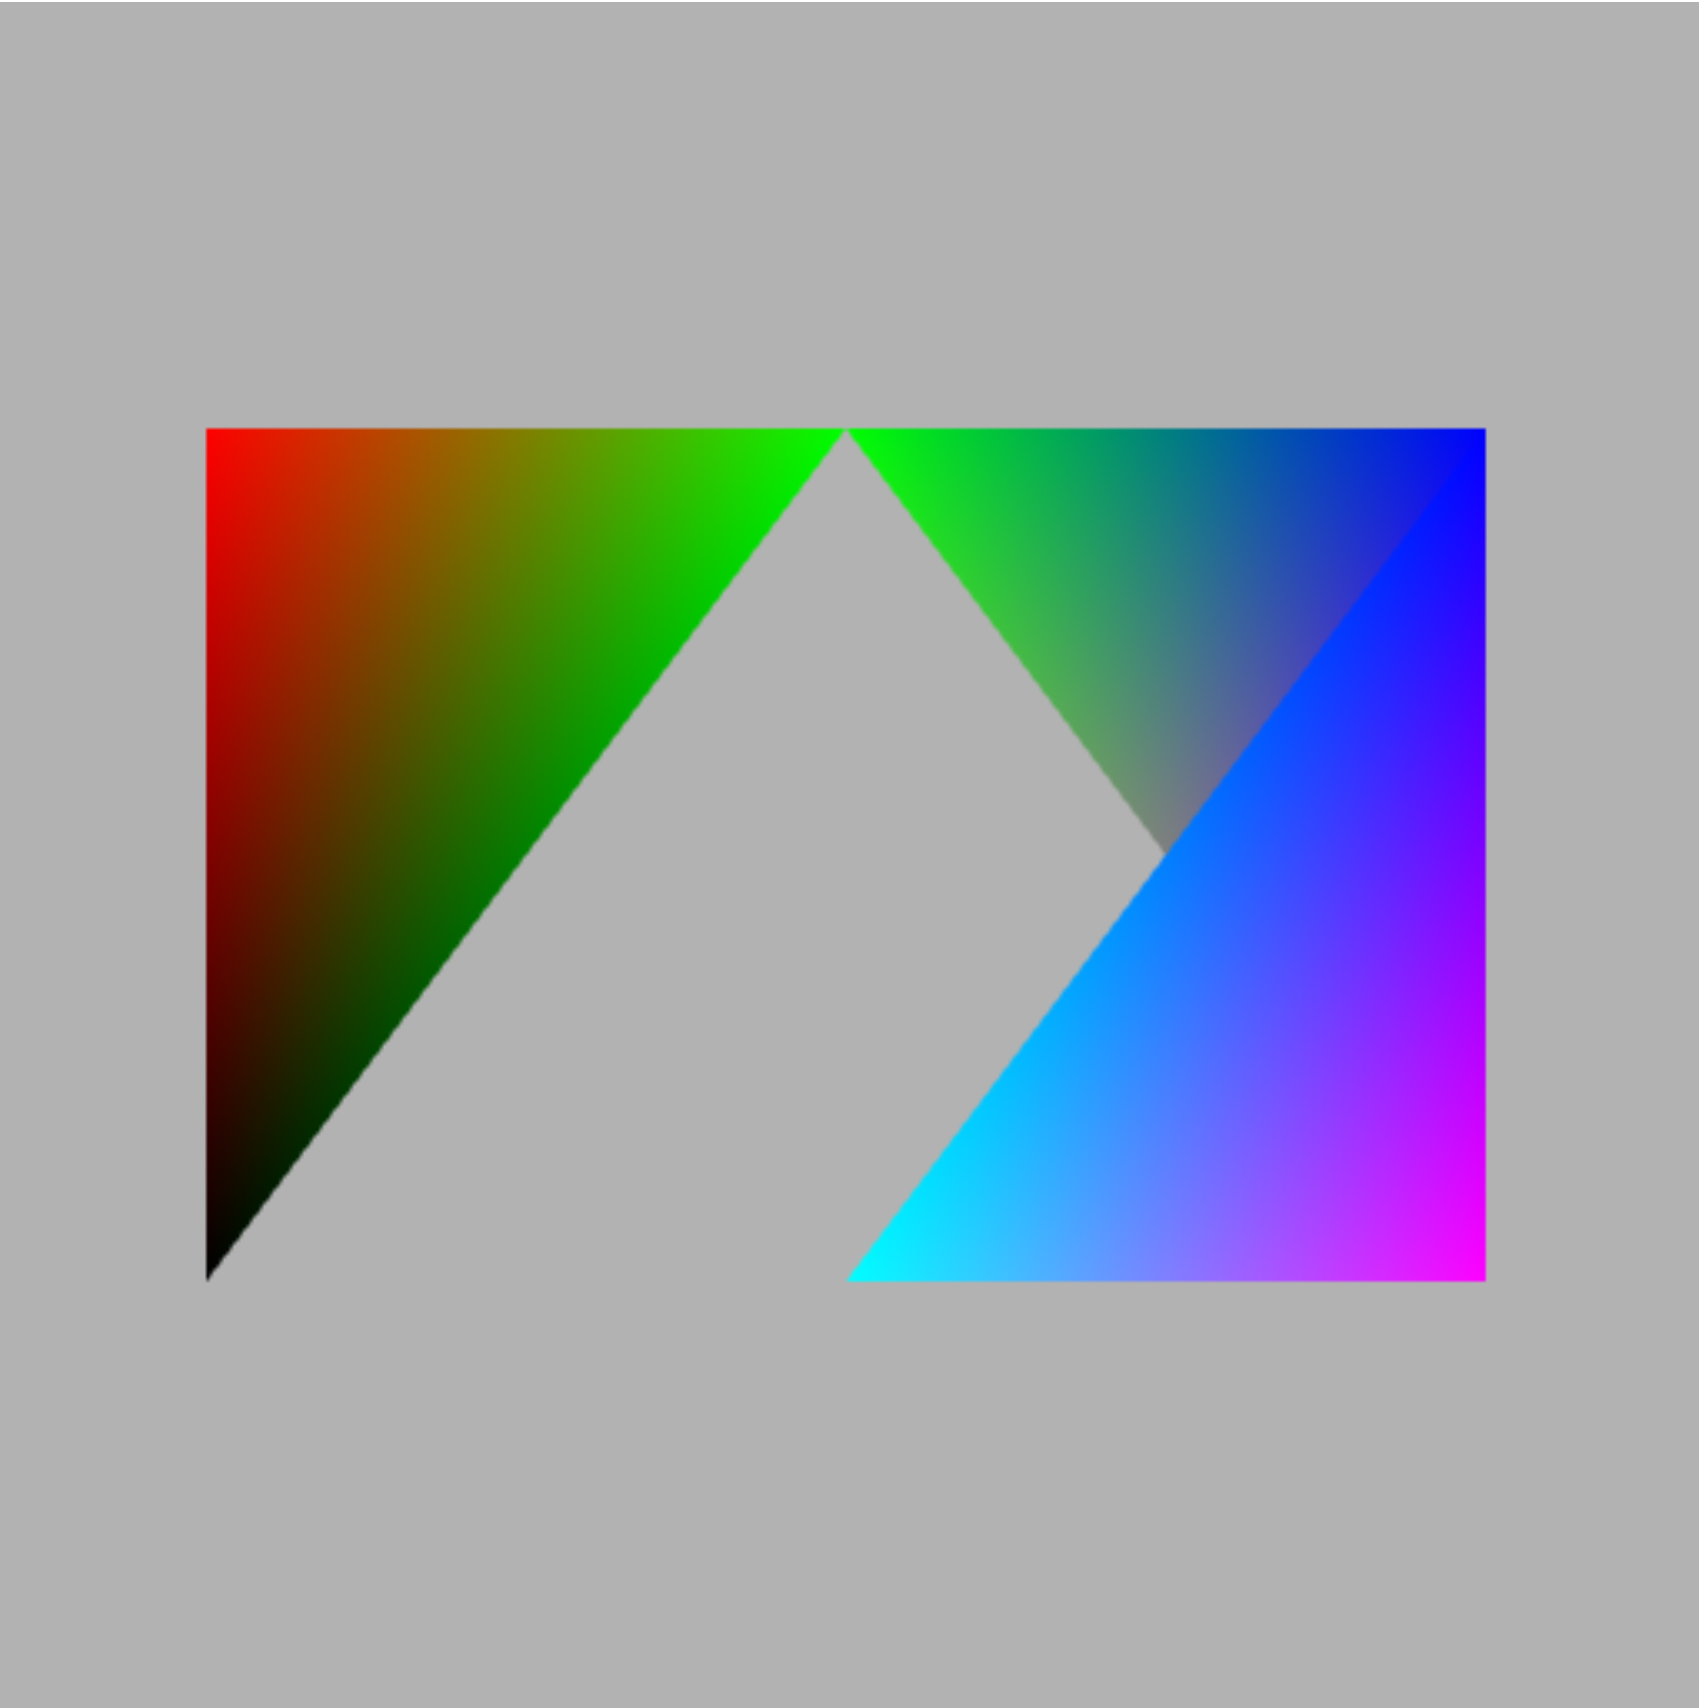
\includegraphics[width=1.0\textwidth]{Image_6}
\part{Question Six: Shading Language}
\section{Question}
\section{Answer}
\part{Question Seven: Projection Transformations}
\section{Question}
\section{Answer}
\part{Question Eight: Lighting Geometry}
\section{Question}
\section{Answer}
\part{Question Nine: Texture Sampling Modes}
\section{Question}
\section{Answer}
\part{Question Ten}
\section{Question}
What feature when using images for textures in OpenGL makes use of reduced size images in areas where the texture image is larger than the area being covered?
\section{Answer}
You can use glPixelZoom() to reduce the size of images in areas where the texture image is larger than the area being covered.
\end{document}